\documentclass[a4paper,twoside,french,11pt]{VcCours}
% cSpell:disable
\newcommand{\dx}{\text{d}x}
\newcommand{\dt}{\text{d}t}

\makeatletter
\NewEnviron{ptc}[2][]{\@Enonce{Point de cours}{methodes}{#2}{%
  \draw (mabox.north west) -- (mabox.south west); 
  \draw[dashed,transform canvas={xshift = 2pt}] (mabox.north west) -- (mabox.south west); 
  \draw[transform canvas={xshift = 4pt}] (mabox.north west) -- (mabox.south west); 
}{#1}{\BODY}{MethodeColor}{black!5}}
\makeatother

% cSpell:enable
\begin{document}
\Titre{PSI}{Promotion 2021--2022}{Mathématiques}{Devoir de vacances de Mathématiques.}

Le but de ce devoir de vacances est de réviser les bases du cours de première année et les méthodes fondamentales associées. Il est primordial d'arriver en deuxième année avec un cours connu, de bonnes bases de calcul et une connaissance de nombreux exercices classiques et méthodes usuelles.

\textit{Extrait du rapport de e3a PSI 2016} : \og Un certain nombre de copies montre une méconnaissance profonde du cours et, à contrario, les candidats qui le maîtrisent peuvent ainsi obtenir de très bonnes notes \fg .

Chacun a sa propre méthode de travail mais voici une manière de procéder durant les vacances :

\begin{enumerate}
\item Tout d'abord réviser son cours et il y a du travail car celui-ci est très dense ! Vous pouvez utiliser vos programmes de colles qui listent les points-clés du cours, les preuves à Connaître (\textit{et à retravailler}) et des exercices classiques. \textit{C'est la partie la plus importante des révisions}.
\item Une fois le premier point fait, vous pouvez vous entraîner à l'aide des exercices de ce devoir maison. La plupart des exercices sont des applications directes du cours ou de méthodes usuelles. Ainsi, si le premier point est bien travaillé, les exercices doivent se traiter sans problème. Vous trouverez des indications (à utiliser \textit{après} avoir réfléchi au problème) dans le document \og Devoir de vacances : éléments de correction \fg .
\item Si vous souhaitez vous entraîner sur des exercices plus compliqués : vous pouvez retravailler vos DM et DS ou me contacter : je vous en enverrai avec grand plaisir !
%\item Pour la rentrée, je vous demande de traiter trois exercices sur feuilles que vous trouverez à la fin de ce document. 
\item Pour les $5/2$ : vous pouvez rajouter le point 1 en utilisant vos programmes de colles de PSI.
\end{enumerate}

Quelques précisions concernant la rentrée : les premiers chapitres concerneront des rappels d'analyse, les séries numériques puis des révisions d'algèbre linéaire : je vous conseille de réviser en priorité pendant les dernières semaines d'août votre cours sur les séries ainsi que les chapitres concernant l'algèbre linéaire (espaces vectoriels, applications linéaires, matrices et déterminants).

Dernier point pour finir : travailler sérieusement ce devoir vous permettra de commencer l'année dans les meilleures conditions. Une soixantaine d'exercices sur deux mois ne demandent pas un si gros sacrifice. 

\begin{center}
 \boxed{\textbf{Important}}
\end{center}

\begin{center}
\textbf{Il y aura un devoir surveillé  le samedi de la rentrée constitué des exercices et des points de cours de ce DM.}
\end{center}

Si vous avez besoin de me contacter : maxime-bailleul@laposte.net. N'hésitez-pas !

% cSpell:disable
\section{Keep calm and do more calculus}
% cSpell:enable

\textit{Extrait du rapport de CCP PSI 2016} : \og Les résultats faibles semblent dus ($\ldots$) à un manque de maîtrise presque total du calcul \fg .

Il est très important de savoir calculer rapidement et sans commettre de faute. Pour cela, il n'y pas de secret : s'entraîner régulièrement sur du calcul \og bête et méchant \fg et Connaître tous les résultats usuels utilisables en pratique : coefficients binomiaux et formule du binôme de Newton, sommes usuelles, primitives et dérivées usuelles, développements limités usuels en $0$, équivalents usuels en $0$, méthodes de résolution d'une équation différentielle linéaire d'ordre $1$ ou d'ordre $2$, méthodes d'obtention du terme général d'une suite arithmético-géométrique  ou d'une suite récurrente linéaire d'ordre $2$.

\subsection{Coefficients binomiaux et formule du binôme}

\begin{ptc}{}
	Connaître la formule de Pascal et une preuve de celle-ci.
\end{ptc}

\begin{ptc}{}
	Connaître la formule du binôme de Newton et une preuve de celle-ci.
\end{ptc}

%
%\begin{Exercice}{}
  %\begin{enumerate}
    %\item Énoncer et démontrer la formule de Pascal. 
    %\item Énoncer et démontrer la formule du binôme de Newton. 
  %\end{enumerate}    
%\end{Exercice} 

\begin{Exercice}{}
  Soit $n \in \mathbb{N}^*$. Calculer les sommes suivantes : 
  $$ \sum_{k=0}^n 2^k \binom{n}{k} \quad \hbox{ et } \quad \sum_{k=0}^n (-1)^k \binom{n}{k}$$
\end{Exercice} 

\subsection{Nombres complexes, trigonométrie et fonctions associées}

\textit{Extrait du rapport de CCP PSI 2016} : \og Tout ce qui est du domaine du calcul (trigonométrie élémentaire parfois utile rappelons-le, développements limités ...) donne lieu à des prestations lentes, faibles, avec des résultats souvent grossièrement faux \fg .

\begin{ptc}{}
	Connaître parfaitement les fonctions $\cos$, $\sin$, $\tan$ $\arcsin$, $\arccos$, $\arctan$ :
\begin{itemize}
\item Ensembles de définition.
\item Ensembles de dérivabilité et dérivées. 
\item Valeurs particulières (savoir utiliser le cercle trigonométrique).
\item Courbes représentatives.
%\item Formules de trigonométries usuelles.
\item Formules de trigonométrie usuelles $\cos(a+b)$, $\cos(2a)$, $\cos(p)\cos(q)$, $\cos(p)+\cos(q)$ $\ldots$
\item Savoir résoudre des équations du type $\cos(a)= \cos(b)$ et $\sin(a)=\sin(b)$.
\end{itemize}
\end{ptc}
%
%\begin{Exercice}{}
%\end{Exercice} 
%Faire une fiche concernant les fonctions cos, sin, tan, arcsin, arcos et arctan résumant les résultats suivants : ensemble de définition, ensemble de dérivabilité et dérivée, valeurs particulières, courbes représentatives, formules de trigonométrie usuelles ($\cos(a+b)$, $\cos(p)\cos(q)$ $\ldots$).

\begin{Exercice}{}
  Calculer $\cos \left(\dfrac{\pi}{8}\right) \cdot$
\end{Exercice} 

\begin{ptc}{}
	Connaître l'expression des racines $n$-ièmes de l'unité. Savoir retrouver très rapidement celles-ci pour $n=3$ et $n=4$.
\end{ptc}

\begin{Exercice}{}
  On note $j=e^{i\tfrac{2\pi}{3}}$. Donner la valeur de $1+j+j^2$.
\end{Exercice} 

\begin{Exercice}{}
  Résoudre $\cos(2x - \tfrac{\pi}{3}) = \sin(x + \tfrac{3\pi}{4})$ d'inconnue $x \in \mathbb{R}$.
\end{Exercice} 

\begin{Exercice}{}
  Montrer que pour tout $x \in \mathbb{R}_+$, $\sin x \leq x$.
\end{Exercice} 

%%
%\begin{Exercice}{}
%A l'aide du théorème de bijection monotone et du théorème de dérivabilité d'une bijection réciproque, démontrer que la fonction $\cos$ est bijective de $[0,\pi]$ sur $[-1,1]$, que sa bijection réciproque (arcos) est dérivable sur $]-1,1[$ et que pour tout $x \in ]-1,1[$,
%\end{Exercice} 
%$$ \arccos'(x) = \frac{-1}{\sqrt{1-x^2}}$$

\begin{Exercice}{}
  Déterminer, pour tout $x \in \mathbb{R}^*$, une expression simple de $\textrm{arctan}(x)+ \textrm{arctan}(1/x)$.
\end{Exercice} 

\begin{Exercice}{}
  Soit $f$ la fonction définie par $f(x) =  \arcsin \left( \frac{x}{\sqrt {1 + x^{2}}} \right) \cdot$

  \begin{enumerate}
    \item Justifier que $f$ est définie sur $\mathbb{R}$.
    \item Donner une expression simple de $f$.
  \end{enumerate}
\end{Exercice} 

\subsection{Sommes}

\begin{ptc}{}
Soient $n \in \mathbb{N}$ et $q \in \mathbb{R}$. Connaître les valeurs des sommes suivantes :
$$ \sum_{k=0}^n k, \;  \sum_{k=0}^n k^2, \; \sum_{k=0}^n k^3  \; \hbox{ et } \; \sum_{k=0}^n q^k$$
\end{ptc}

\begin{Exercice}{}
  Avez-vous oublié le cas $q=1$ dans le dernier point de cours ?
\end{Exercice} 

\begin{Exercice}{}
  Soient $n \in \mathbb{N}^*$ et $\omega $ une racine $n$-ième de l'unité. Déterminer la valeur de la somme $S_n$ définie par :$$ S_n= \sum_{k=0}^{n-1} \omega^k$$
\end{Exercice} 

\begin{Exercice}{}
  \begin{enumerate}
    \item Montrer que pour tout $\alpha \in \mathbb{R}$, $e^{i \alpha}-1 = 2ie^{i \frac{\alpha}{2}}\sin \left(\frac{\alpha}{2}\right)$ (\textit{égalité classique à retrouver rapidement}).
    \item Déterminer pour tout $n \in \mathbb{N}^*$ et $x \in ]0, 2\pi [$ les valeurs de :
    $$ \sum_{k=0}^n \cos(kx) \quad \hbox{ et }  \quad\sum_{k=0}^n \sin(kx) $$
  \end{enumerate}
\end{Exercice} 

\subsection{Dérivées et primitives}

\textit{Extrait du rapport CCP PSI 2016} : \og Les calculs de primitives, même simples, posent des difficultés à nombre de candidats \fg{} .

\begin{ptc}{}
	Connaître parfaitement les dérivées et primitives usuelles, la formule d'intégration par parties et la formule de changement de variables.
\end{ptc}

\begin{Exercice}{}
  Donner les primitives des fonctions suivantes (il suffit de trouver de trouver la primitive \og à vue \fg $u'e^{u}$, $u'u^n$ etc... sauf pour la dernière ou il suffit de linéariser) :

  \begin{multicols}{2}
    \begin{enumerate}
      \item $x \mapsto xe^{-x^2}$ sur $\mathbb{R}$.
      \item $x \mapsto \dfrac{\ln(x)}{x}$ sur $\mathbb{R}_{+}^*$.
      \item $x \mapsto \dfrac{1}{x\ln(x)}$ sur $]0,1[$ puis sur $]1, + \infty[$.
      \columnbreak
      \item $x \mapsto \dfrac{e^{2x}}{\sqrt{1-e^{2x}}}$ sur $\mathbb{R}_{-}^*$.
      \item $x \mapsto \dfrac{\tan^2(x)+1}{\sqrt{\tan(x)}}$ sur $\mathbb{R}_{+}^*$.
      \item $x \mapsto \cos(x)^3$.
    \end{enumerate}
  \end{multicols}
\end{Exercice} 

\begin{Exercice}{}
  Calculer à l'aide d'intégration(s) par parties :

  \begin{multicols}{2}
    \begin{enumerate}
      \item $I= \int_{1}^e \ln(x) \dx$.
      \item $J= \int_{0}^1 x^2 e^x \dx$.
      \item $K = \int_{0}^{1} \arctan(x) \dx$.
      \columnbreak
      \item $L = \int_{0}^{\pi/2} (-x+5) \sin(2x) \dx$.
      \item $M = \int_{0}^1 \sin(x) e^x \dx$.
    \end{enumerate}
  \end{multicols}
\end{Exercice} 

\begin{Exercice}{}
  Calculer les intégrales suivantes à l'aide d'un changement de variable :
  $$I= \int_{0}^1 \dfrac{e^{2t}}{e^t+1} \dt, \; J = \int_{1}^e \dfrac{\ln(t)}{t+t\ln(t)^2} \dt \; \hbox{ et } K = \int_{0}^1 \dfrac{1}{e^x+1} \dx$$
\end{Exercice} 

\begin{Exercice}{}
  Pour tout entier naturel $n$, on pose $I_{n}=\int_{1}^{e}x^{2}\ln \left( x\right) ^{n}dx$.
  \begin{enumerate}
    \item  Calculer $I_0$.
    \item 
    \begin{enumerate}
      \item Étudier le sens de variation de la suite $(I_{n})_{n \geq 0}$.

      \item  Montrer que la suite $(I_{n})_{n \geq 0}$ est convergente.

      \item  Montrer que pour tout $x\in [1,e], \, 0 \leq \ln (x) \leq x/e$.

      \item  En déduire que $\lim\limits_{n\rightarrow +\infty }I_{n}=0$.
    \end{enumerate}
    \item 
    \begin{enumerate}
      \item  Montrer que pour tout entier naturel $\displaystyle n$, 
      $$I_{n+1}={
        \frac{e^{3}}{3}}-{\frac{n+1}{3}}I_{n}$$

        \item  En déduire un équivalent de $I_n$ quand $n$ tend vers $+ \infty$.        
    \end{enumerate}
  \end{enumerate}
\end{Exercice} 

\begin{Exercice}{}
  Étudier la dérivabilité de $H : x \mapsto \int_x^{x^2} e^{-t^2} \dt$.
\end{Exercice} 

\subsection{Équations différentielles}

\begin{ptc}{}
	Savoir étudier une équation différentielle linéaire du premier ordre à coefficient et second membre continues :
\begin{itemize} 
\item Résolution de l'équation homogène.
\item Obtention d'une solution particulière (méthode de la variation de la constante).
\item Forme des solutions : somme d'une solution particulière et de la solution générale de l'équation homogène.
\item Existence et unicité du problème de Cauchy
\end{itemize}
\end{ptc}

\begin{ptc}{}
	Savoir étudier une équation différentielle linéaire du second ordre à coefficients constants :
\begin{itemize} 
\item Résolution de l'équation homogène.
\item Obtention d'une solution particulière si le second membre a une forme particulière.
\item Forme des solutions : somme d'une solution particulière et de la solution générale de l'équation homogène.
\item Existence et unicité du problème de Cauchy.
\end{itemize}
\end{ptc}

\begin{Exercice}{}
  Résoudre les équations différentielles suivantes : 

  \begin{enumerate}
    \item $y'-xy=x\,\exp(x^2)$ sur $\mathbb{R}$.
    \item $\cos(x)y'+ \sin(x)y=1$ sur $]-\pi/2, \pi/2[$.
    \item $y'+y=\dfrac{1}{1+\exp(x)}$ sur $\mathbb{R}$.
  \end{enumerate}
\end{Exercice} 

\begin{Exercice}{}
  Résoudre les équations différentielles suivantes :

  \begin{multicols}{2}
    \begin{enumerate}
      \item $2y''+5y'-3y=0$.
      \item $y''- 3y' + 3y=0$.
      \columnbreak
      \item $y''-2y'+y=0$.
      \item $y''-4y'+3y=e^x$.
    \end{enumerate}
  \end{multicols}
\end{Exercice} 

\subsection{Développements limités}

\begin{ptc}{}
	Connaître les développements limités usuels et les équivalents usuels en $0$.
\end{ptc}
%
%\begin{Exercice}{}
%\end{Exercice} 
%Faire une fiche résumant les résultats suivants : développements limités usuels en $0$, équivalents usuels en $0$.
%
%

Si l'on connaît le développement limité d'une fonction $f$ en $0$ et que l'on souhaite obtenir le développement de $f \circ g$ en $0$, on peut substituer si quand $x$ tend vers $0$, $g(x)$ tend vers $0$. Si ce n'est pas le cas, on peut parfois utiliser propriétés suivantes :
$$ \exp(b+g(x)) = \exp(b) \exp(g(x)), \; \ln(b+g(x))= \ln(b)+ \ln \left( 1 + \frac{g(x)}{b} \right), \; \frac{1}{b+g(x)} = \frac{1}{b}\frac{1}{1+ \frac{g(x)}{b}}$$

\begin{Exercice}{}
  Donner les développements limités suivants : 

  \begin{multicols}{2}
    \begin{enumerate}
      \item $\cos(x) \ch(x)$ à l'ordre $4$ en $0$.
      \item $\ln(1+x)(1-\cos(x))$ à l'ordre $4$ en $0$.
      \item $\ln(1+ \sin(x))$ à l'ordre $3$ en $0$.
      \columnbreak
      \item $\sqrt{x}$ à l'ordre $2$ en $2$.
      \item $\ln(1 + \sqrt {1 + x})$ à l'ordre $3$ en $0$.
      \item $\dfrac{1}{1+\ch(x)}$ à l'ordre $3$ en $0$.
    \end{enumerate}
  \end{multicols}
\end{Exercice} 

\begin{Exercice}{}
  Déterminer les équivalents suivants :

  \begin{multicols}{2}
    \begin{enumerate}
      \item $\sqrt{x^3+1} \sin \left( \dfrac{1}{x}\right)$ en $+ \infty$.
      \item $\ln(\cos(x))$ en $0$.
      \item $\ln(x^2+3x+2)$ en $+ \infty$.
      \columnbreak
      \item $x\ln(x)+1$ en $0$.
      \item $x(2 + \cos x) - 3\sin x$ en $0$.
      \item $\ln( \cos(x))$ en $\dfrac{\pi}{2}\cdot$
    \end{enumerate}
  \end{multicols}
\end{Exercice} 

\begin{Exercice}{}
  Déterminer $\lim_{n \rightarrow + \infty} \left( 1+ \frac{1}{n} \right)^n$ et $\lim_{n \rightarrow + \infty} \left( 1+ \frac{1}{n} \right)^{n^2}\cdot$
\end{Exercice} 

\subsection{Suites usuelles}

\begin{ptc}{}
	Savoir déterminer le terme général d'une suite arithmético-géométrique et d'une suite récurrente linéaire d'ordre deux.
\end{ptc}

\begin{Exercice}{}
  Déterminer le terme général des suites définies de la manière suivante :

  \begin{enumerate}
    \item $u_0=2$ et pour tout $n \in \mathbb{N}$, $u_{n+1} = 5 u_n -6$. 
    \item $v_0=1$ et pour tout $n \in \mathbb{N}$, $2v_{n+1}= v_n+ 4$.
  \end{enumerate}
\end{Exercice} 

\begin{Exercice}{}
  Déterminer le terme général des suites \textit{réelles} définies de la manière suivante :
  \begin{enumerate}
    \item $u_0=u_1=1$ et pour tout $n \in \mathbb{N}$ par $u_{n+2}=3u_{n+1}-u_n$.
    \item $u_0=u_1=1$ et pour tout $n \in \mathbb{N}$ par $u_{n+2}-2u_{n+1}+u_n=0$.
    \item $u_0=0$, $u_1=1$ et pour tout $n \in \mathbb{N}$ par $u_{n+2}=u_{n+1}-u_n$.
  \end{enumerate}
\end{Exercice}

\section{Études de suites et de fonctions}

\begin{ptc}{}
	Connaître la définition du cosinus et du sinus hyperbolique et des équivalents en $+ \infty$ et $- \infty$ de celles-ci :
$$ \forall x \in \mathbb{R}, \; \textrm{ch}(x) = \dfrac{e^x+e^{-x}}{2} \; \hbox{ et } \; \textrm{sh}(x) = \dfrac{e^x-e^{-x}}{2}$$
\end{ptc}

\begin{ptc}{}
	Savoir montrer qu'une fonction est prolongeable par continuité, est dérivable en un point.
\end{ptc}

\begin{Exercice}{}
  Soit $f$ la fonction définie par $f(x) = x^2 \sin \left( \frac{1}{x} \right) \cdot$

  \begin{enumerate}
    \item Justifier que $f$ est dérivable sur son ensemble de définition.
    \item Montrer que $f$ est prolongeable par continuité en $0$. Montrer que ce prolongement est dérivable en $0$.
  \end{enumerate}
\end{Exercice} 

\begin{Exercice}{}
  Étudier la convergence de la suite définie par un premier terme $u_0 \in \mathbb{R}_+^*$ et pour tout entier $n \geq 0$ par $u_{n+1} = \dfrac{u_n}{u_n^2+1} \cdot$
\end{Exercice} 

\begin{ptc}{}
	Connaître les multiples versions du théorème des valeurs intermédiaires.
\end{ptc}

\begin{Exercice}{}
  Soit $f$ une fonction continue sur $[0,1]$ à valeurs dans $[0,1]$. Montrons que $f$ admet au moins un point fixe.
\end{Exercice} 

\begin{Exercice}{}
  Montrer que tout polynôme réel de degré impair admet au moins une racine réelle.
\end{Exercice} 

\begin{ptc}{}
	Connaître le théorème de bijection monotone et le théorème de dérivabilité d'une bijection réciproque.
\end{ptc}

\begin{Exercice}{}
  Soit $f$ la fonction définie pour tout réel $x>0$ par :
  $$ f(x)= x+ \ln(x)$$
  Montrer que $f$ réalise une bijection de $\mathbb{R}_+^{*}$ sur un intervalle $J$ à déterminer. La bijection réciproque de $f$ est-elle dérivable sur $J$ ?
\end{Exercice} 

\begin{ptc}{}
	Connaître le théorème de Rolle, l'égalité des accroissements finis et l'inégalité des accroissements finis.
\end{ptc}

\begin{Exercice}{}
  Montrer que pour tout $x>0$,
  $$ \dfrac{1}{x+1} < \ln \left( 1 + \dfrac{1}{x} \right) < \dfrac{1}{x}$$
\end{Exercice} 

\begin{Exercice}{}
  Soit $f$ la fonction définie pour tout $x \in I=[1, + \infty[$ par $f(x) = \frac{x}{1+\ln(x)} \cdot$
  
  \begin{enumerate}
    \item
    \begin{enumerate}
      \item Montrer que pour tout $x \in I$, $f(x) \in I$.
      \item Résoudre l'équation $f(x)=x$ d'inconnue $x \in I$.
      \item Donner un encadrement de $f'$ sur $I$.
    \end{enumerate}
    \item Soit $(u_n)_{n \geq 0}$ la suite définie par $u_0=2$ et pour tout $n \geq 0$ par $u_{n+1}=f(u_n)$.
    \begin{enumerate}
      \item Justifier que $(u_n)_{n \geq 0}$ est bien définie.
      \item Montrer que pour tout $n\geq 0$, $\vert u_{n+1} - 1 \vert \leq \frac{1}{4} \vert u_n - 1 \vert$.
      \item En déduire que pour tout $n \geq 0$, $\vert u_n - 1 \vert \leq \dfrac{1}{4^n}\cdot$ Qu'en déduit-on?
    \end{enumerate}
  \end{enumerate}
\end{Exercice} 
  
\begin{Exercice}{} 
  \begin{enumerate}
    \item Montrer que pour tout $x \in ]0, + \infty[$,
    \[ \frac{1}{2\sqrt{x+1}} \leq \sqrt{x+1} - \sqrt{x} \leq \frac{1}{2\sqrt{x}} \]
    \item En déduire que pour tout $n \in \mathbb{N}^*$, $\sqrt{n+1} - 1 \leq \frac{1}{2} \sum_{k=1}^n \frac{1}{\sqrt{k}} \cdot$
    \item Étudier la nature de $\sum_{n \geq 1} \frac{1}{\sqrt{n}} \cdot$
  \end{enumerate}
\end{Exercice} 
  
  \begin{ptc}{}
    Connaître la formule de Leibniz concernant la dérivée $n$-ième d'un produit de fonctions ainsi qu'une preuve de celle-ci.
  \end{ptc}

\begin{Exercice}{}
\end{Exercice} 
\begin{enumerate}
\item
On pose $g(x)=\mathrm{e}^{2x}$ et $h(x)=\dfrac{1}{1+x} \cdot$\\
Calculer, pour tout entier naturel $k$, la dérivée d'ordre $k$ des fonctions $g$ et $h$ sur leurs ensembles de définitions respectifs.
\item 
On pose $f(x)=\dfrac{\mathrm{e}^{2x}}{1+x}\cdot$\\
En utilisant la formule de Leibniz, concernant la dérivée $n^{\text{ème}}$ d'un produit de fonctions, déterminer, pour tout entier naturel $n$ et pour $x\in\mathbb{R}\backslash\left\lbrace -1\right\rbrace $, la valeur de $f^{n}(x)$.
\end{enumerate}

\section{Séries}

\begin{ptc}{}

\begin{itemize}
\item Connaître la définition de série, sommes partielles.
\item Connaître la définition de convergence et divergence d'une série.
\item Savoir que le terme général d'une série convergente tend vers $0$. La réciproque est fausse : série harmonique.
\end{itemize}
\end{ptc}

\begin{Exercice}{}
  Étudier la convergence de $\sum_{n \geq 1} \ln \left( 1 + \dfrac{1}{n} \right) \cdot$
\end{Exercice} 

\begin{ptc}{}
	Connaître parfaitement les séries géométriques :
\begin{itemize}
\item Expression des sommes partielles.
\item Condition nécessaire et suffisante de convergence.
\item Somme en cas de convergence.
\end{itemize}
\end{ptc}

\begin{Exercice}{}
  Étudier la convergence de $\sum_{n \geq 1} \dfrac{2^n}{3^{n+1}}$ et donner sa somme en cas de convergence.
\end{Exercice} 

\begin{ptc}{}
	Connaître les séries de Riemann et le critère de convergence associé.
\end{ptc} 

\begin{ptc}{}
	Savoir montrer qu'une série converge avec les critères suivants : 
\begin{itemize}
\item Critère de comparaison des séries à termes positifs : $u_n \leq v_n$ et $u_n \underset{+ \infty}{\sim} v_n$.
\item La convergence absolue implique la convergence (pratique pour se ramener à une série à termes positifs).
\item Critère du type $u_n \underset{+ \infty}{=} O (v_n)$.
\end{itemize}
\end{ptc}

\begin{Exercice}{}
  Étudier la convergence des séries $\sum u_n$ dans les cas suivants :
  
  \begin{multicols}{3}
    \begin{enumerate}
      \item $u_n = \dfrac{1}{n^3+n^2+n}$
      \item $u_n = \dfrac{2n^2+n}{3n^3+n}$
      \columnbreak
      \item $u_n = \dfrac{1}{n} \sin \left( \dfrac{1}{n} \right)$
      \item $u_n = \dfrac{\sin(n)}{n^2} $
      \columnbreak
      \item $u_n = n^2 e^{-n}$
      \item $u_n = (-1)^n e^{-n^2}$
    \end{enumerate}
  \end{multicols}
\end{Exercice} 

\section{Polynômes}

\begin{ptc}{}
	Connaître la formule de Taylor pour les polynômes.
\end{ptc}

%\begin{Exercice}{}
  % Effectuer la division euclidienne de $X^5-X^4-2X^2-3X+1$ par $X^2+2$.
% \end{Exercice} 

%Q=X^3-2X-1 et R=2X

\begin{Exercice}{}
  Soit $P \in \mathbb{R}[X]$. Montrer que si $\int_0^1 P(t)^2 \dt= 0$ alors $P$ est le polynôme nul.
\end{Exercice} 

\begin{Exercice}{}
  Soit $P \in \mathbb{C}[X]$ tel que $P(X+1)=P(X)$. Montrer que $P$ est constant.
\end{Exercice} 

\begin{Exercice}{}
  Pour tout $n \geq 1$, posons :
  $$ P_n(X) = n X^{n+2} - (n+2)X^{n+1} + (n+2)X -n $$
  \begin{enumerate}
    \item Calculer $P_n(1)$, $P_n'(1)$ et $P_n''(1)$.
    \item Qu'en déduit-on ?
  \end{enumerate}
\end{Exercice} 
  
\begin{ptc}{}
	Connaître les polynômes irréductibles de $\mathbb{C}[X]$ et de $\mathbb{R}[X]$.
\end{ptc}

\begin{Exercice}{}
  
  \begin{enumerate}
    \item Factoriser dans $\mathbb{C}[X]$ le polynôme $X^2+X+1$.
    \item Factoriser dans $\mathbb{C}[X]$ le polynôme $X^4+X^2+1$.
  \end{enumerate}
\end{Exercice} 
  
\section{Algèbre linéaire}

\textit{Extrait du rapport de CCP PSI 2016} : \og Les espaces vectoriels, les sommes directes, trop souvent même, le théorème du rang posent problème à de nombreux candidats \fg .

\textit{Extrait du rapport de e3a PSI 2016 : (en parlant de questions liées à l'algèbre linéaire de première \newline année) } : \og Leur traitement est très décevant dans beaucoup de questions \fg .

\subsection{Sous-espaces vectoriels}

\begin{ptc}{}
	Soit $E$ un $\mathbb{K}$-espace vectoriel, $F \subset E$ et $x_1$, $\ldots$, $x_p$ des vecteurs de $E$ ($p \geq 1$). Connaître parfaitement :
\begin{itemize}
\item La définition de sous-espace vectoriel de $F$.
\item La définition de $\textrm{Vect}(x_1, \ldots, x_p)$ et la preuve que c'est un sous-espace vectoriel de $E$.
\end{itemize}
\end{ptc}

%\begin{center}
%\textbf{{\Large Partie 1 : Algèbre linéaire}}
%\end{center}
%
%%
%
%$\rhd$ Savoir repérer rapidement des sous-ensembles n'étant pas des sous-espaces vectoriels.
%
%$\rhd$ Savoir montrer qu'un sous-ensemble $F$d'un espace vectoriel $E$ est un sous-espace vectoriel par la méthode des trois points : le vecteur nul de $E$ appartient à $F$, stabilité par la somme et stabilité par le produit externe (que l'on peut regrouper en une étape).
%
%$\rhd$ Savoir montrer qu'un sous-ensemble $F$ d'un espace vectoriel $E$ est un sous-espace vectoriel engendré (ce qui nous donne directement une famille génératrice, il reste alors à étudier la liberté de cette famille pour obtenir éventuellement une base).
%
%$\rhd$ Savoir montrer qu'une somme de sous-espaces est une somme directe et savoir montrer que deux espaces sont supplémentaires.
%
%$\rhd$ Connaître parfaitement la notion de famille libre, famille génératrice, base.
%
%

\begin{Exercice}{}
  Justifier rapidement que les sous-ensembles suivants ne sont pas des sous-espaces vectoriels de $\mathbb{R}^2$ :
  
  \begin{enumerate}
    \item $F_1 = \lbrace (x,y) \in \mathbb{R}^2 \, \vert \, x+y=1 \rbrace $
    \item $F_2 = \lbrace (x,y) \in \mathbb{R}^2 \, \vert xy=0 \rbrace $
  \end{enumerate}
\end{Exercice} 

\begin{Exercice}{}
  L'ensemble des fonctions croissantes sur $\mathbb{R}$ est-il un sous-espace vectoriel de l'espace vectoriel\footnote{Remarquons que nous ne rappelons quasiment jamais les lois de compositions associées aux espaces vectoriel usuels.} des fonctions définies sur $\mathbb{R}$ à valeurs dans $\mathbb{R}$?
\end{Exercice} 

\begin{Exercice}{}
  Montrer que les sous-ensembles $F$ suivants sont des sous-espaces vectoriels de $E$ :
  
  \begin{enumerate}
    \item $E$ l'ensemble des fonctions continues sur $[0,1]$ à valeurs dans $\mathbb{R}$ et $F$ l'ensemble défini par :
    $$ F = \left\lbrace f \in E \, \big{\vert} \, \int_{0}^1 f(t) \dt =0 \right\rbrace$$
    \item $E$ l'ensemble des matrices carrées d'ordre $n \geq 1$ et $F$ l'ensemble défini par :
    $$  F = \left\lbrace M \in E \, \big{\vert} \, AM=MA \right\rbrace$$
    où $A$ est une matrice carrée fixée de $E$.
  \end{enumerate}
\end{Exercice} 
  
\begin{ptc}{}
	Soient $E$ un $\mathbb{K}$-espace vectoriel et $F$,$G$, deux-sous espaces vectoriels de $E$. Connaître parfaitement la définition de :
\begin{itemize}
\item $F$ et $G$ sont en somme directe.
\item $F$ et $G$ sont supplémentaires dans $E$.
\end{itemize}
\end{ptc}

\begin{Exercice}{}
  Montrer que l'ensemble des fonctions paires et l'ensemble des fonctions impaires sont des espaces supplémentaires de l'espace vectoriel des fonctions de $\mathbb{R}$ dans $\mathbb{R}$. On raisonnera par analyse-synthèse pour déterminer la décomposition d'une fonction.
\end{Exercice} 

\subsection{Familles libres, génératrices, bases}

\begin{ptc}{}
	Connaître parfaitement la définition de famille libre, famille génératrice, base.
\end{ptc}

\begin{Exercice}{}
  Écrire les sous-ensembles suivants comme des sous-espaces vectoriels engendrés puis donner une base de ces espaces :
  
  \begin{enumerate}
    \item $A=\lbrace (x,y,z) \in \mathbb{R}^3 \, \vert  \, 2x-y+z=0 \rbrace \cdot$
    \item $B= \lbrace (x,y,z) \in \mathbb{R}^3 \, \vert \, z+y=0 \rbrace \cdot$
    \item $C= A \cap B.$
    \item $D = \lbrace P \in \mathbb{R}_4[X], P(0)=P'(0)=P'(1)=0 \rbrace \cdot$
  \end{enumerate}
\end{Exercice} 
  
\begin{Exercice}{}
  La famille $((1,1,0), \, (2,1,-3), \, (1,0,1))$ est-elle libre dans $\mathbb{R}^3$?
\end{Exercice} 

\begin{Exercice}{}
  Soit $n \in \mathbb{N}$. Justifier rapidement que la famille $\mathcal{F}$ définie par :
  $$ \mathcal{F} = (1, (X-1), (X-1)^2, (X-1)^3, \ldots, (X-1)^n)$$
  est une famille libre de $\mathbb{R}[X]$.
\end{Exercice} 
  
\begin{Exercice}{}
  Montrer que la famille $(\cos, \sin)$ est une une famille libre de l'espace vectoriel des fonctions de $\mathbb{R}$ dans $\mathbb{R}$.
\end{Exercice} 

\begin{Exercice}{}
  Soit $f : \mathbb{R} \rightarrow \mathbb{R}$ définie par $f(x)=e^x$. Montrer que $(f,f^2,f^3)$ est une famille libre de l'espace vectoriel des fonctions de $\mathbb{R}$ dans $\mathbb{R}$.
\end{Exercice} 

\subsection{Dimension finie}

\begin{ptc}{}
	Soit $E$ un $\mathbb{K}$-espace vectoriel de dimension finie et $F$, $G$ deux sous-espaces de $E$
\begin{itemize}
\item Savoir qu'une famille de $E$ est libre si et seulement si elle est génératrice si et seulement si c'est une base.
\item Connaître la formule de Grassman.
\item Connaître la dimension d'une somme directe de deux sous-espace.
\item Savoir que $F$ et $G$ sont supplémentaires si et seulement si $F \cap G = \lbrace 0_E \rbrace$ et $\textrm{dim}(E)= \textrm{dim}(F) + \textrm{dim}(G)$.
\item Connaître la définition du rang d'une famille de vecteurs.
\end{itemize}
\end{ptc}

\begin{Exercice}{}
Montrer que $F=\textrm{Vect}((1,0,0,1), \, (0,0,1,0))$ et $G=\textrm{Vect}((0,0,0,1), \, (0,1,0,1))$ sont deux sous-espaces supplémentaires de $\mathbb{R}^4$.
\end{Exercice} 

\begin{Exercice}{}
  Déterminer un supplémentaire de $\lbrace P(X) \in \mathbb{R}_4[X], \, P(-X)=P(X)\rbrace$ dans $\mathbb{R}_4[X]$.
\end{Exercice} 

\begin{Exercice}{}
  Déterminer le rang de la famille $(x_1,x_2,x_3)$ de vecteurs de $\mathbb{R}^4$ où
  $$ x_1 = (1,1,1,1), \, x_2 = (1, - 1,1, - 1), \, x_3 = (1,0,1,1)$$
\end{Exercice} 
  
\subsection{Applications linéaires (sans les matrices)}

Soient $\mathbb{K}= \mathbb{R}$ ou $\mathbb{C}$ et $E, F$ deux $\mathbb{K}$-espaces vectoriels. On note $\mathcal{L}(E,F)$ l'ensemble des applications linéaires de $E$ dans $F$. Si $E=F$, on note simplement $\mathcal{L}(E)$ (qui est donc l'ensemble des endomorphismes de $E$).

\begin{ptc}{}

\begin{itemize}
\item Connaître la définition d'application linéaire, d'endomorphisme, d'isomorphisme, d'automorphisme.
\item Soit $f \in \mathcal{L}(E,F)$. Connaître la définition du noyau et de l'image de $f$. Savoir montrer que ce sont des sous-espaces vectoriels (de $E$ pour le noyau, de $F$ pour l'image).
\item Soit $f \in \mathcal{L}(E,F)$. Si $(e_1, \ldots, e_n)$ est une base de $E$,
$$ \textrm{Im}(f) = \textrm{Vect}(f(e_1), \ldots, f(e_n))$$
\item Connaître la définition de rang d'une application linéaire et le théorème du rang.
\end{itemize} 
\end{ptc}
%
%\begin{Exercice}{}
  %Soit $f \in \mathcal{L}(E,F)$. Redonner la définition du noyau et de l'image de $f$. Montrer que ce sont des sous-espaces vectoriels (de $E$ pour le noyau, de $F$ pour l'image).
%\end{Exercice} 

\begin{Exercice}{}
  Soit $f : \mathbb{R}^3 \rightarrow \mathbb{R}^3$ définie par :
  $$ \forall (x,y,z) \in \mathbb{R}^3, \; f((x,y,z))= (x+2y+z,y-x,2x+4y+z)$$
  Montrer que $f$ est un automorphisme de $\mathbb{R}^3$.
\end{Exercice} 

\begin{Exercice}{}
  Soit $f : \mathbb{R}^3 \rightarrow \mathbb{R}^3$ définie par :
  $$ \forall (x,y,z) \in \mathbb{R}^3, \; f((x,y,z))= (x+z,x+z,x+y)$$
  Montrer que $f$ est un endomorphisme de $\mathbb{R}^3$. Déterminer une base du noyau et une base de l'image de $f$.
\end{Exercice} 

\begin{Exercice}{}
  Soient $I$ un intervalle de $\mathbb{R}$ contenant au moins deux points,  $\mathcal{C}^1(I, \mathbb{R})$ l'ensemble des fonctions de classes $\mathcal{C}^1$ sur $I$ à valeurs dans $\mathbb{R}$ et $\mathcal{F}(I, \mathbb{R})$ l'ensemble des fonctions définies sur $I$ et à valeurs dans $\mathbb{R}$. 
  
  Soit $\varphi : \mathcal{C}^1(I, \mathbb{R}) \rightarrow \mathcal{F}(I, \mathbb{R})$ définie par :
  $$ \forall f \in \mathcal{C}(I, \mathbb{R}), \; \varphi(f)=f'$$
  
  \begin{enumerate}
    \item Montrer que $\varphi \in \mathcal{L}(\mathcal{C}^1(I, \mathbb{R}),\mathcal{F}(I, \mathbb{R}))$.
    \item L'application $\varphi$ est-elle injective? Surjective ?
    \item Déterminer le noyau et l'image de $\varphi$.
  \end{enumerate}
\end{Exercice} 

\begin{Exercice}{}
  Soient $n \geq 1$ et $a_{0} ,a_{1} , \ldots ,a_{n}$ des éléments deux à deux distincts de $\mathbb{C}$. Montrer que l'application $\varphi \colon \mathbb{C}_n[X] \rightarrow \mathbb{C}^{n+1}$ définie par
  \[\varphi(P) = (P(a_{0}),P(a_{1}), \ldots ,P(a_{n}))\]
  est un isomorphisme.
\end{Exercice} 
    
\begin{Exercice}{}
  Soit $f \in \mathcal{L}(E)$. Montrer les inclusions suivantes :
  
  \begin{enumerate}
    \item $\textrm{Ker}(f) \subset \textrm{Ker}(f^2)$.
    \item $\textrm{Im}(f^2) \subset \textrm{Im}(f)$.
  \end{enumerate}
\end{Exercice} 

\begin{Exercice}{}
  Soit $f$ l'application définie sur $\mathbb{R}_2[X]$ par $f(P)=P-(X+1)P'+X^2 P''$.
  \begin{enumerate}
    \item Montrer que $f$ est un endomorphisme de $\mathbb{R}_2[X]$.
    \item Déterminer le noyau de $f$.
    \item Que vaut le rang de $f$? Déterminer une base de l'image de $f$.
  \end{enumerate}
\end{Exercice} 
  
\begin{Exercice}{}
  Soient $\mathbb{K}= \mathbb{R}$ ou $\mathbb{C}$ et $\varphi : \mathbb{K}_{n+1}[X]\rightarrow \mathbb{K}_{n}[X]$ définie par $\varphi(P) = (n + 1)P - XP'$.
  \begin{enumerate}
    \item
    Justifier que $\varphi$ est bien définie et que c'est une application linéaire.
    \item
    Déterminer le noyau de $\varphi$.
    \item
    $\varphi$ est-elle surjective?
  \end{enumerate}
\end{Exercice} 

\begin{ptc}{}
	Connaître la définition de projecteurs et symétries associés à deux sous-espaces supplémentaires et les caractérisations associées ($p \circ p = p$ et $s \circ s = \textrm{Id}$).
\end{ptc} 

\begin{Exercice}{}
  Soient $E= \mathbb{R}^3$ et $F$, $G$ les ensembles définis par :
  $$ F = \lbrace (x,y,z) \in \mathbb{R}^3, \, x-y+z=0 \rbrace \quad \hbox{ et }  \quad G = \textrm{Vect}((1,1,1)) $$
  
  \begin{enumerate}
    \item Donner une base de $F$ et préciser sa dimension.
    \item Montrer que $F$ et $G$ sont supplémentaires.
    \item Soit $p$ la projection sur $F$ parallèlement à $G$. Donner l'expression de $p$.
    \item Soit $q$ la projection sur $G$ parallèlement à $F$. Donner\footnote{Si votre réponse dépasse une ligne : relire le point de cours précédent.} l'expression de $q$.
  \end{enumerate}
\end{Exercice} 
  
%%
%\begin{Exercice}{}
  %Soient $q$ et $q$ deux projecteurs d'un espace vectoriel $E$. Montrer que $p$ et $q$ ont le même noyau si et seulement si $p=p \circ q$ et $q=q \circ p$.
%\end{Exercice} 

\begin{Exercice}{}
  Soient la matrice $A= \begin{pmatrix}
    1 & 2 \\
    2 & 4 \\
  \end{pmatrix}$ et $f$ l'endomorphisme de $\mathcal{M}_2(\mathbb{R})$ défini par $f(M)=AM$.
  
  \begin{enumerate}
    \item Déterminer une base de $\textrm{Ker}(f)$.
    \item $f$ est-il surjectif ?
    \item Déterminer une base de $\textrm{Im}(f)$.
    \item A t-on $\mathcal{M}_2(\mathbb{R}) = \textrm{Ker}(f) \oplus \textrm{Im}(f)$ ?
  \end{enumerate}
\end{Exercice} 
  
\subsection{Calcul matriciel}

\begin{Exercice}{}
  Montrer que $P = \begin{pmatrix}
    2 & 1 & 1 \\
    -1 & 2 & -1 \\
    1 & 1 & 1
  \end{pmatrix}$ est inversible et donner sa matrice inverse.
\end{Exercice} 
  
\begin{Exercice}{}
  
  Soit $A = \begin{pmatrix} 4&1&1\\1&4&1\\1&1&4\end{pmatrix} \cdot$
  \begin{enumerate}
    \item Calculer $A^2$ et montrer qu'il existe deux réels $\alpha$ et $\beta$ tels que $A^2 = \alpha A + \beta I_3$.
    \item En déduire que $A$ est inversible et exprimer $A^{-1}$.
  \end{enumerate}
\end{Exercice} 
  
\begin{ptc}{}
	Connaître la formule du binôme pour des matrices (qui \textit{commutent}).
\end{ptc}

\begin{Exercice}{}
  Soit $M = \begin{pmatrix}
    2 & 0 & 1 \\
    0 & 1 & 0 \\
    0 & 0 & 2
  \end{pmatrix}$ et $T= \begin{pmatrix}
    0 & 0 & 1 \\
    0 & 0 & 0 \\
    0 & 0 & 0
  \end{pmatrix}\cdot$
  
  \begin{enumerate}
    \item Déterminer $T^n$ pour tout $n \geq 0$.
    \item En déduire $M^n$ pour tout $n \geq 0$.
  \end{enumerate}
\end{Exercice} 

\subsection{Applications linéaires (avec les matrices)}

\begin{ptc}{}
	Savoir déterminer le noyau, l'image et le rang d'une matrice.
\end{ptc} 

\begin{Exercice}{}
  Donner le noyau, le rang et l'image de $A = \begin{pmatrix}
    -5 & 4 & -1 \\
    -4 & 3 & - 1 \\
    2 	 & -2 & 0 \\
  \end{pmatrix}\cdot$
\end{Exercice} 
  
\begin{ptc}{}
	Savoir déterminer la matrice d'une application linéaire dans des bases données (ou pour un endomorphisme dans une base donnée).
\end{ptc}

\begin{Exercice}{}
  On considère l'application $\varphi : \mathbb{R}_2[X] \rightarrow \mathbb{R}^3$ définie par :
  \[ \varphi(P)=(P(0),P'(0),P(1)) \]
  
  \begin{enumerate}
    \item Déterminer la matrice de $\varphi$ dans les bases canoniques des espaces considérés.
    \item Montrer que $\varphi$ est un isomorphisme d'espaces vectoriels.
    \item Déterminer une expression de $\varphi^{-1}$.
  \end{enumerate}
\end{Exercice} 

\begin{Exercice}{}
  Posons :
  $$ \begin{array}{ccccl}
    f & : & \mathbb{R}_2[X] & \rightarrow & \mathbb{R}_2[X] \\
    & & P & \rightarrow & (X+1)P' \\
  \end{array} $$
  \begin{enumerate}
    \item Montrer que $f$ est un endomorphisme de $ \mathbb{R}_2[X]$.
    \item Déterminer la matrice $M$ de $f$ dans la base canonique $\mathcal{B}$ de $\mathbb{R}_2[X]$.
    \item Considérons la famille suivante : $\mathcal{B}'= (1, (X+1),(X+1)^2)$. Montrer que $\mathcal{B}'$ est une base de $\mathbb{R}_2[X]$ et déterminer la matrice $N$ de $f$ dans cette base.
    \item Déterminer le lien entre $M$ et $N$.
    \item Déterminer les puissances de $M$.
  \end{enumerate}
\end{Exercice} 

\begin{Exercice}{}
  Soit $n \in \mathbb{N}^*$. Pour tout $P \in \mathbb{R}_n[X]$, on pose $\Phi(P)=P(X+1)-P(X-1)$.
  
  \begin{enumerate}
    \item Montrer que $\Phi$ est un endomorphisme de $\mathbb{R}_n[X]$.
    \item Déterminer sa matrice dans la base canonique de $\mathbb{R}_n[X]$.
  \end{enumerate}
\end{Exercice} 

\begin{Exercice}{}
  On considère les sous-espaces vectoriels de $\mathbb{R}^3 $ suivants :
  
  $P = \left\{ {(x,y,z) \in \mathbb{R}^3 \mid x + 2y - z = 0} \right\}$ et $D = \textrm{Vect} (w){\text{ o\`u }}w = (1,0, - 1)$. On note $\mathcal{B}$ la base canonique de $\mathbb{R}^3 $.
  
  \begin{enumerate}
    \item Justifier l'existence de la projection vectorielle sur $P$ parallèlement à $D$. Notons $p$ ce projecteur.
    \item Donner la matrice de $p$ dans ${\mathcal{B}}$.
    \item En déduire les matrices, dans ${\mathcal{B}}$, de la projection vectorielle sur $D$ parallèlement à $P$ et de la symétrie vectorielle par rapport à $P$ et parallèlement à $D$.
  \end{enumerate}
\end{Exercice}
  
\begin{Exercice}{}
  Soit $n \in \mathbb{N}^*$. On note $\mathbb{R}_n[X]$ le $\mathbb{R}$-espace vectoriel des polynômes à coefficients réels de degré inférieur ou égal à $n$. On pose pour tout $P \in \mathbb{R}_n[X]$,
  $$ \varphi_n(P) = P-P'$$
  
  \begin{enumerate}
    \item Démontrer que $\varphi_n$ est un endomorphisme de $\R_n[X]$.
    \item Expliciter la matrice de $ \varphi_n$ dans la base canonique de $\R_n[X]$.
    \item Démontrer que $\varphi_n$ est un automorphisme de $\R_n[X]$.
    \item En déduire qu'il existe une unique famille de polynômes $s_0,s_1,\ldots,s_n$ telle que :
    \begin{enumerate}
      \item $\forall i \in \iii{0}{n}, \  \varphi_n(s_i)=\dfrac{X^i}{i!}$,
      \item $(s_0,s_1,\ldots,s_n)$ est une base de $\R_n[X]$.
    \end{enumerate}
    \item On note $\textrm{Id}$ l'endomorphisme identité de $\R_n[X]$ et $\delta$ l'endomorphisme induit par la dérivation sur le $\R-$espace vectoriel $\R_n[X]$ (c'est-à-dire défini par $\delta(P)=P'$). Justifier que : 
    $$(\textrm{Id}-\delta)\circ (\textrm{Id} +\delta+\cdots+\delta^n)=\textrm{Id}$$
    \item En déduire l'expression de $s_i$, pour tout $i$ dans $\iii{0}{n}$.
  \end{enumerate}
\end{Exercice} 

\subsection{Déterminants}

\begin{Exercice}{}
  Calculer pour $(a,b,c) \in \mathbb{R}^2$,
  $\begin{vmatrix}
    a & b & c \\
    c & a & b \\
    b & c & a
  \end{vmatrix} \cdot$
\end{Exercice} 
  
\begin{Exercice}{}
  Soient $E$ un $\mathbb{R}$-espace vectoriel de dimension 3 et $\mathcal{B}$ une base de $E$. Soit $f$ l'endomorphisme de $E$ dont la matrice dans $\mathcal{B}$ est
  \[
    A=\begin{pmatrix}
      3 & -2 & -3 \\
      -2 & 6 & 6 \\
      2 & -2 & -2
    \end{pmatrix}
  \]
  \begin{enumerate}
    \item Pour quelles valeurs de $\lambda$, a-t-on $\textrm{det} ( A - \lambda I_{3} ) = 0$? \textit{On utilisera des opérations élémentaires pour essayer d'obtenir une forme factorisée lors du calcul du déterminant.}
    \item Soient $\lambda_1$, $\lambda_2$ et $\lambda_3$ les trois réels obtenus (dans l'ordre croissant). Déterminer pour tout $i \in \lbrace 1,2,3 \rbrace$, une base du noyau de $f -\lambda_i \textrm{Id}_E$. En concaténant les bases obtenues, justifier que l'on obtient une base de $E$ et déterminer la matrice de $f$ dans cette nouvelle base.
  \end{enumerate}
\end{Exercice} 
    
\begin{Exercice}{}
  Soit $n \in \mathbb{N}^{*}$. Calculer
  \[
    \begin{vmatrix}
      S_{1} & S_{1} & S_{1} & \cdots & S_{1} \\
      S_{1} & S_{2} & S_{2} & \cdots & S_{2} \\
      S_{1} & S_{2} & S_{3} & \cdots & S_{3} \\
      \vdots & \vdots & \vdots & \ddots & \vdots \\
      S_{1} & S_{2} & S_{3} & \cdots & S_{n}
    \end{vmatrix}
  \]
  où pour tout $ k \in \iii{1}{n}$, on a $ S_{k} = \sum_{i = 1}^{k} i $.
\end{Exercice} 
    
    %
    %
    %\section{Exercices à rendre le jour de la rentrée}
%
%%
%Les exercices suivants sont à rendre le jour du premier cours de mathématiques. Le point important à comprendre est qu'\textit{il ne sert strictement à rien de recopier sur quelqu'un ou de recopier un corrigé}. Les devoirs maisons doivent se traiter en condition concours : seul. Concernant les trois exercices : les deux premiers sont calculatoires ou rappellent des méthodes usuelles. L'exercice 3 est un extrait d'un sujet e3a. Il n'est pas dramatique de ne pas savoir traiter une question : passez-la au besoin mais il sera dans ce cas important d'étudier le corrigé à la rentrée.
%
%
%
%Vous \fbox{encadrerez} ou \underline{soulignerez} vos résultats.
%
%
%
%
%
%\textit{\textbf{Exercice 1 : un peu de calcul...}}
%
% Pour tout réel $m$, on définit la fonction 
%$$ f_m : x \mapsto e^{2x} + m \ln(1-x) \cos(x)$$
%de courbe représentative notée $\mathcal{C}_m$.
%
%\begin{enumerate}
%\item Déterminer le développement limité de $f_m$ à l'ordre $3$ en $0$.
%\item Donner l'équation de la tangente de $\mathcal{C}_m$, notée $\mathcal{T}_m$, au point d'abscisse $0$.
%\item Peut-on trouver un réel $m$ pour lequel la tangente $\mathcal{T}_m$ soit parallèle à l'axe des abscisses ? Si oui, tracer dans ce cas l'allure de $\mathcal{C}_m$ au voisinage de $0$.
%\item Peut-on trouver un réel $m$ pour lequel la tangente $\mathcal{T}_m$ soit parallèle à la droite d'équation $y=-x$ ? 
%\end{enumerate}
%
%
%%
%%\begin{Exercice}{}
  % Pour tout entier $n$ supérieur ou égal à $3$, on pose pour tout $x \in [0,1]$, $f_n(x)=x^n+1-nx.$
  % \end{Exercice} 
%%\begin{enumerate}
%%\item Étudier pour tout entier $n \geq 3$, les variations de la fonction $f_n$ sur $[0,1]$.
%%\item Montrer que pour tout entier $n \geq 3$, l'équation $x^n+1=nx$ possède une unique solution dans l'intervalle $]0,1[$. On la note $x_n$.
%%\item Montrer que pour tout entier $n \geq 3$, $\displaystyle{\frac 1 n < x_n < \frac 2 n}\cdot$\\
%%Que peut-on en déduire sur la convergence de la suite $(x_n)_{n \ge 3}$ ?
%%\item Montrer que $x_n \underset{+\infty}{\sim}\dfrac{1}{n}\cdot$
%%\item Montrer que $\lim_{n \rightarrow + \infty} (1 + x_n^n)=1$.
%%\item En déduire un équivalent simple de $x_n - \dfrac{1}{n}$ puis un développement asymptotique de $x_n$ à deux termes.
%%\end{enumerate}
%
%
%
%
%
%
%
%\textit{\textbf{Exercice 2 : méthodes de bases en algèbre linéaire.}}
%
%Considérons les ensembles suivants :
%$$ F = \lbrace (x,y,z) \in \mathbb{R}^3 \, \vert \, y=z \rbrace \quad \hbox{ et } \quad G = \lbrace (x,y,z) \in \mathbb{R}^3 \, \vert \, x-y=0 \hbox{ et } z-2y=0 \rbrace$$
%
%\begin{enumerate}
%\item 
%\begin{enumerate}
%\item Donner une base de $F$.
%\item Donner une base de $G$.
%\item Montrer que $F$ et $G$ sont supplémentaires.
%\end{enumerate}
%\item Soit $u=(x,y,z) \in \mathbb{R}^3$.
%\begin{enumerate}
%\item Donner l'unique décomposition de $u$ dans $F \oplus G$.
%\item En déduire l'expression de la projection sur $F$ parallèlement à $G$.
%\item Donner l'expression de la symétrie par rapport à $F$ parallèlement à $G$.
%\end{enumerate}
%\end{enumerate}
%
%
%
%%%%
%%\begin{Exercice}{}
%   Soient $n$ un entier naturel non nul et $E$ un $\mathbb{R}$-espace vectoriel de dimension $n$. On dit qu'un endomorphisme $f$ de $E$ est cyclique si il existe un vecteur $x$ de $E$ tel que $(x,f(x),f^2(x), \ldots, f^n(x))$ soit une base de $E$.
% \end{Exercice} 
%%
%%%%
%%\begin{enumerate}
%%\item \textit{Un exemple.} On considère dans cette question que $E = \mathbb{R}^2$. Soit $g$ l'endomorphisme de $E$ dont la matrice dans la base canonique est la matrice 
%%$$ A = \begin{pmatrix}
%%4  & -6 \\
%%1 & -1 \\
%%\end{pmatrix}$$
%%\begin{enumerate}
%%\item Soit $x=(2,3)$. Déterminer $g(x)$ puis montrer que $g$ est cyclique.
%%\item Déterminer deux réels $\alpha$ et $\beta$ tels que :
%%$$ g^2(x)= \alpha x + \beta g(x)$$
%%\item Donner la matrice de $f$ dans la base $(x,g(x))$.
%%\end{enumerate}
%%%%\item \textit{Un autre exemple.} On considère dans cette question que $E = \mathbb{R}_{n-1}[X]$ où $n$ est un entier supérieur ou égal à $2$. Soit $h$ l'endomorphisme de $E$ qui à tout polynôme $P$ associée $P'$.
%%\begin{enumerate}
%%\item Pour tout entier $k$ tel que $1 \leq k \leq n-1$, déterminer $g^k(X^{n-1})$.
%%\item En déduire que $h$ est cyclique.
%%\end{enumerate}
%%
%%%%
%%\item \textit{Un résultat général.} Soient $E$ un espace vectoriel de dimension $n \geq 2$ et $f$ un endomorphisme de $E$ : c'est-à-dire qu'il existe un entier naturel non nul $n$ tel que $f^n$ soit l'endomorphisme nul.
%%
%%\begin{enumerate}
%%\item On appelle indice de nilpotence de $f$ le plus petit entier naturel $k$ tel que $f^k$ soit l'endomorphisme nul. Justifier l'existence de celui-ci. On le notera $s$.
%%\item Justifier l'existence d'un vecteur $x$ de $E$ tel que $f^{s -1}(x)$ soit différent du vecteur nul.
%%\item Montrer que $f$ est cyclique.
%%\end{enumerate}
%%\end{enumerate}
%
%%
%%\section{Annexes : quelques méthodes, rédactions usuelles...}
%%
%%\subsection{Projecteur, projection et symétrie}
%%
%%Soient $E$ un $\mathbb{K}$-espace vectoriel et $F$, $G$ deux sous-espaces vectoriels supplémentaires de $E$.
%%
%%Pour tout $x \in E$, il existe un unique couple $(x_F,x_G) \in F \times G$ tel que $x=x_F+x_G$. On pose $p(x)=x_F$. On définit ainsi une application $p : E \rightarrow E$ que l'on appelle projection vectorielle sur $F$ parallèlement à $G$. 
%%
%%\begin{center}
%%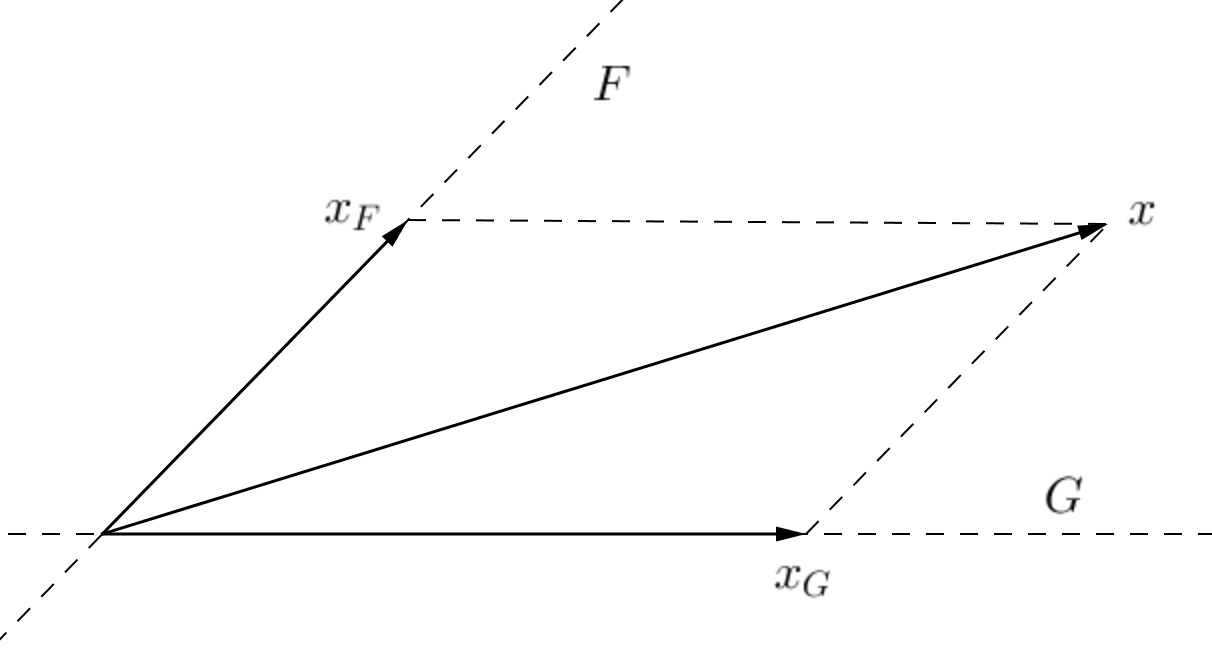
\includegraphics[scale=0.4]{Projection1}
%%\end{center}
%%
%%On a alors les propriétés suivantes :
%%\begin{itemize}
%%\item $p$ est un endomorphisme de $E$.
%%\item $\textrm{Im}(p) = \textrm{ker}(p-id)$ et $\textrm{Ker}(p)=G$.
%%\item Pour tout $x \in E$, $x=p(x)+x-p(x)$ où $p(x) \in \textrm{Ker}(p-id)$ et $x-p(x) \in \textrm{Ker}(p)$
%%\item Un endomorphisme $p$ de $E$ est une projection si et seulement si $p \circ p = p$. Dans ce cas, $p$ est une projection sur $\textrm{ker}(p-id)$ parallèlement à $\textrm{ker}(p)$.
%%\end{itemize}
%%
%%\begin{metho} Pour montrer que deux sous-espaces vectoriels $F$ et $G$ d'un espace vectoriel $E$ de dimension finie sont supplémentaires, on peut utiliser l'une des assertions suivantes (équivalentes) :
%%\begin{itemize}
%%\item Pour tout $x \in E$, il existe un unique couple $(x_F,x_G) \in F \times G$ tel que $x=x_F+x_G$.
%%\item $E=F+G$ et $F \cap G = \lbrace 0_E \rbrace$.
%%\item $\textrm{dim}(E)= \textrm{dim}(F) + \textrm{dim}(G)$ et $F \cap G = \lbrace 0_E \rbrace$ (méthode la plus simple).
%%\end{itemize}
%%L'avantage de la première méthode est de donner la décomposition de tout vecteur $x$ (et donc l'expression de la projection sur $F$ ou sur $G$).
%%\end{metho}
%%
%%
%%\textbf{Exemple.} On considère les sous-espaces vectoriels de $\mathbb{R}^3 $ suivants : $P = \left\{ {(x,y,z) \in \mathbb{R}^3 \mid x + 2y - z = 0} \right\}$ et $D = \textrm{Vect} (w){\text{ o\`u }}w = (1,0, - 1)$. Justifier l'existence de la projection vectorielle, notée $p$, sur $P$ parallèlement à $D$ puis donner son expression.
%%
%%%%
%%\textbf{\textit{Première idée :}}
%%
%%Montrons que $P$ et $D$ sont supplémentaires en raisonnant par analyse-synthèse :
%%
%%$\rhd$ \textit{Analyse} : Soit $x=(x,y,z) \in \mathbb{R}^3$. On suppose qu'il existe $(x_P,x_D) \in P \times D$ tel que $x=x_P+x_D$. Par définition de $P$, $x_p=(a,b,c)$ où $a+2b-c=0$ et par définition, il existe $\alpha \in \mathbb{R}$ tel que $x_D= \alpha (1,0,-1)$. Ainsi :
%%$$ (x-\alpha, y, z + \alpha) = (a,b,c)$$
%%et donc :
%%$$ x- \alpha + 2y- (z + \alpha) = 0$$
%%ce qui implique $\alpha = \dfrac{x+2y-z}{2}$ puis $x_D =  \dfrac{x+2y-z}{2}(1,0,-1)$ et donc $x_P = x-\dfrac{x+2y-z}{2} (1,0,-1)$.
%%
%%%%
%%$\rhd$ \textit{Synthèse} : Soit $x =(x,y,z) \in \mathbb{R}^3$. Posons :
%%$$ x_D =  \dfrac{x+2y-z}{2}(1,0,-1) \quad \hbox{ et } x_P = x-x_D$$
%%On a bien $x=x_D+x_P$. Il est clair que $x_D \in D$. Vérifions que $x_P \in P$ : on a :
%%$$ x_P = (x,y,z)  -\dfrac{x+2y-z}{2} (1,0,-1) = \left(x- \dfrac{x+2y-z}{2}, y, z+ \dfrac{x+2y-z}{2} \right)$$
%%et :
%%$$ x- \dfrac{x+2y-z}{2} + 2y - \left( z+ \dfrac{x+2y-z}{2} \right) = 0$$
%%donc $x_P \in P$. Tout vecteur de $\mathbb{R}^3$ est donc somme d'un élément de $D$ et d'un élément de $P$ et cette décomposition est unique (d'après l'analyse).
%%
%%%%
%%Ainsi $P$ et $D$ sont supplémentaires dans $\mathbb{R}^3$ donc la projection de vectorielle sur $P$ paraallèlement à $D$ existe. Le raisonnement nous fournit son expression : 
%%$$ \forall (x,y,z) \in \mathbb{R}^3, \, p((x,y,z))= \left(x- \dfrac{x+2y-z}{2}, y, z+ \dfrac{x+2y-z}{2} \right) = \dfrac{1}{2} \left(x-2y+z , 2y, x+2y+z \right)$$
%%
%%%%
%%\textbf{\textit{Deuxième idée :}} si l'on souhaite juste montrer que $P$ et $D$ sont supplémentaires, on peut raisonner autrement.
%%
%%\begin{itemize}
%%\item Soit $(x,y,z) \in \mathbb{R}^3$. On a $(x,y,z) \in P$ si et seulement si $x+2y-z=0$ ou encore $x=-2y+z$ et finalement si et seulement si $(x,y,z) = (-2y+z,y,z) = y(-2,1,0)+z(1,0,1)$. Ainsi $P = \textrm{Vect}((-2,1,0),(1,0,1))$ et $P$ est de dimension $2$ car les des vecteurs sont non colinéaires. De plus, $D$ est de dimension $1$ (car $(1,0,-1)$ est non nul). Ainsi :
%%$$ \boxed{\textrm{dim}(\mathbb{R}^3) = \textrm{dim}(P) + \textrm{dim}(D)}$$
%%\item $D$ est de dimension $1$ (car $(1,0,-1)$ est non nul).
%%\item Soit $(x,y,z) \in D \cap P$. Par définition, il existe $\alpha \in \mathbb{R}$ tel que $(x,y,z)= \alpha (1,0,-1)$ et $x+2y-z=0$
%%\end{itemize}
%%
%%
%%
%
%
%
%\textit{\textbf{Exercice 3 : extrait de concours e3a.}}
%
%Soit $n$ un entier naturel non nul.
%\begin{enumerate}
%\item Soit $\theta\in [0,2\pi[$. Déterminer, s'ils existent, module et argument du nombre complexe $u=1+e^{i\theta}$.
%\item On note $P_n$ le polynôme de $\C[X]$ défini par
%\[P_n(X)=\frac{1}{2i}\left ((X+i)^{2n+1}-(X-i)^{2n+1}\right )\]
%\begin{enumerate}
%\item \textit{Étude des cas $n=1$ et $n=2$.}
%\begin{enumerate}
%\item Déterminer les polynômes $P_1$ et $P_2$.
%\item Vérifier que $P_1\in \R_2[X]$ et que $P_2\in \R_4[X]$. Sont-ils irréductibles dans $\R[X]$~?
%\end{enumerate}
%\item \textit{Cas général.}
%\begin{enumerate}
%\item Montrer que $P_n\in \C_{2n}[X]$. Donner son degré et son coefficient dominant.
%\item Soit $N\in \N^*$. Donner l'expression des racines $N$-i\`emes de l'unité.
%\item Calculer $P_n(i)$.
%\item Prouver par un argument géométrique que les racines de $P_n$ sont réelles.
%\item Soit $a\in \C$. Montrer l'équivalence suivante : 
%\begin{center}
%$a$ est racine de $P_n$ $\iff$ $\exists k\in \iii{1}{2n}$, $ \quad a (e^{2ik\pi/(2n+1)}-1)=i(e^{2ik\pi/(2n+1)}+1)$
%\end{center}
%\item Déterminer les racines du polynôme $P_n$. Vérifier alors le résultat de 2(b).iv.
%\item En développant $P_n$, déterminer un polynôme $Q_n$ de degré $n$ et \`a coefficients réels tel que
%\[P_n(X)=Q_n(X^2)\]
%On admettra l'unicité du polynôme $Q_n$ ainsi obtenu.
%\item Expliciter $Q_1$ et $Q_2$ et déterminer leurs racines respectives.
%\item Déterminer les racines de $Q_n$ en fonction de celles de $P_n$.
%\end{enumerate}
%\end{enumerate}
%\item On pose $S_n=\displaystyle \sum_{k=1}^n\frac{1}{\tan^2\left (\frac{k\pi}{2n+1}\right )} \cdot$ En utilisant des résultats obtenus \`a la question précédente, montrer que $S_n=\dfrac{n(2n-1)}{3}\cdot$
%\item Illustrer graphiquement les inégalités suivantes que l'on admettra :
%\[\forall x\in \left [0,\frac{\pi}{2}\right [,\ 0\leq \sin(x)\leq x\leq \tan(x)\]
%En déduire que
%\[\forall x\in \left ]0,\frac{\pi}{2}\right [,\ \frac{1}{\tan^2(x)}\leq \frac{1}{x^2}\leq 1+\frac{1}{\tan^2(x)}\]
%\item Justifier la convergence de la série de terme général $\dfrac{1}{k^2}$ et calculer la somme $\sum_{k=1}^\infty \frac{1}{k^2} \cdot$
%\end{enumerate}
%
%
%
%

\end{document}